\cmfnewsection{Visualização de Resultados: Alguns Detalhes}{./logos/fundo_tese}{0.15}




%%%%%%%%%%%%%%%%%%%%%%%%%%%%%%%%%%%%%%%%%%%%%%%%
%%%%%%%%%%%%%%%%%%%%%%%%%%%%%%%%%%%%%%%%%%%%%%%%
%%%%%%%%%%%%%%%%%%%%%%%%%%%%%%%%%%%%%%%%%%%%%%%%
%%%%%%%%%%%%%%%%%%%%%%%%%%%%%%%%%%%%%%%%%%%%%%%%
\begin{frame}{Ajustes nos Gráficos: Curvas}
\centering

\begin{columns}
\column{0.3\linewidth}

\begin{itemize}
\item É possível selecionar qual curva mostrar
\vspace*{2cm}
\item É possível selecionar aumentar a espessura da curva
\end{itemize}


\column{0.7\linewidth}
\centering
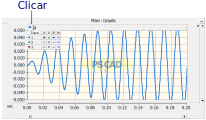
\includegraphics[width=0.9\linewidth]{./figuras/Visualizacao-resultados/graficos-Selecao}

\end{columns}

\end{frame}





%%%%%%%%%%%%%%%%%%%%%%%%%%%%%%%%%%%%%%%%%%%%%%%%
%%%%%%%%%%%%%%%%%%%%%%%%%%%%%%%%%%%%%%%%%%%%%%%%
%%%%%%%%%%%%%%%%%%%%%%%%%%%%%%%%%%%%%%%%%%%%%%%%
%%%%%%%%%%%%%%%%%%%%%%%%%%%%%%%%%%%%%%%%%%%%%%%%
\begin{frame}{Ajustes nos Gráficos: Escala}
\centering

\begin{columns}
\column{0.3\linewidth}

\begin{itemize}
\item Propriedades do gráfico
\vspace*{1cm}
\item Permite ajustar a escala
\vspace*{1cm}
\item Permite alterar a grade
\end{itemize}


\column{0.7\linewidth}
\centering
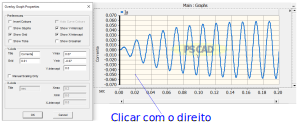
\includegraphics[width=0.9\linewidth]{./figuras/Visualizacao-resultados/graficos-escalas}

\end{columns}

\end{frame}





%%%%%%%%%%%%%%%%%%%%%%%%%%%%%%%%%%%%%%%%%%%%%%%%
%%%%%%%%%%%%%%%%%%%%%%%%%%%%%%%%%%%%%%%%%%%%%%%%
%%%%%%%%%%%%%%%%%%%%%%%%%%%%%%%%%%%%%%%%%%%%%%%%
%%%%%%%%%%%%%%%%%%%%%%%%%%%%%%%%%%%%%%%%%%%%%%%%
\begin{frame}{Ajustes nos Gráficos: Atalhos}

Depois de clicar no gráfico:
\vspace*{1cm}
\begin{itemize}
\item \textbf{E} - Ajusta a escala do tempo
\vspace*{0.75cm}
\item \textbf{Y} - Ajusta a escala y do gráfico para melhor visualização
\vspace*{0.75cm}
\item \textbf{B} - Ajusta a escala y do gráfico de acordo com a configuração do output chanel
\vspace*{0.75cm}
\item \textbf{M} - Habilita dois cursores 
\end{itemize}

\end{frame}




%%%%%%%%%%%%%%%%%%%%%%%%%%%%%%%%%%%%%%%%%%%%%%%%
%%%%%%%%%%%%%%%%%%%%%%%%%%%%%%%%%%%%%%%%%%%%%%%%
%%%%%%%%%%%%%%%%%%%%%%%%%%%%%%%%%%%%%%%%%%%%%%%%
%%%%%%%%%%%%%%%%%%%%%%%%%%%%%%%%%%%%%%%%%%%%%%%%
\begin{frame}{Ajustes nos Gráficos: Polygrphs}
\centering

\begin{columns}
\column{0.3\linewidth}

\begin{itemize}
\item Propriedades do gráfico
\vspace*{1cm}
\item Permite ajustar a escala
\vspace*{1cm}
\item Permite alterar a grade
\end{itemize}


\column{0.7\linewidth}
\centering
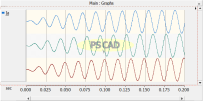
\includegraphics[width=0.9\linewidth]{./figuras/Visualizacao-resultados/graficos-polygraph}

\end{columns}

\end{frame}





%%%%%%%%%%%%%%%%%%%%%%%%%%%%%%%%%%%%%%%%%%%%%%%%
%%%%%%%%%%%%%%%%%%%%%%%%%%%%%%%%%%%%%%%%%%%%%%%%
%%%%%%%%%%%%%%%%%%%%%%%%%%%%%%%%%%%%%%%%%%%%%%%%
%%%%%%%%%%%%%%%%%%%%%%%%%%%%%%%%%%%%%%%%%%%%%%%%
\begin{frame}{Ajustes nos Gráficos: adicionando curvas ao gráfico}
\centering


\begin{columns}
\column{0.25\linewidth}

\begin{itemize}
\item Selecione o {\it output chanel}
\vspace*{1cm}
\item Precione a tecla {\it CTRL}
\vspace*{1cm}
\item Arraste em direção a um gráfico existente
\end{itemize}


\column{0.75\linewidth}
\centering
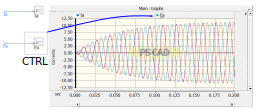
\includegraphics[width=0.95\linewidth]{./figuras/Visualizacao-resultados/graficos-add-curvas}

\end{columns}





\end{frame}






%%%%%%%%%%%%%%%%%%%%%%%%%%%%%%%%%%%%%%%%%%%%%%%%
%%%%%%%%%%%%%%%%%%%%%%%%%%%%%%%%%%%%%%%%%%%%%%%%
%%%%%%%%%%%%%%%%%%%%%%%%%%%%%%%%%%%%%%%%%%%%%%%%
%%%%%%%%%%%%%%%%%%%%%%%%%%%%%%%%%%%%%%%%%%%%%%%%
\begin{frame}{Ajustes nos Gráficos: Painéis de Controle}
\centering



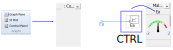
\includegraphics[width=0.95\linewidth]{./figuras/Visualizacao-resultados/graficos-Control-panel}




\end{frame}








%
%
%
%%%%%%%%%%%%%%%%%%%%%%%%%%%%%%%%%%%%%%%%%%%%%%%%%
%%%%%%%%%%%%%%%%%%%%%%%%%%%%%%%%%%%%%%%%%%%%%%%%%
%%%%%%%%%%%%%%%%%%%%%%%%%%%%%%%%%%%%%%%%%%%%%%%%%
%%%%%%%%%%%%%%%%%%%%%%%%%%%%%%%%%%%%%%%%%%%%%%%%%
%\begin{frame}{Ajustes nos Gráficos: Medidor Fasorial}
%\centering
%
%
%\end{frame}



